\documentclass[11pt]{article}

\usepackage{fullpage}
\usepackage{fourier}
\usepackage{euler}
\usepackage{amsmath}
\usepackage{graphicx}
\usepackage{xspace}
\usepackage{epigraph}
\usepackage{listings}
\usepackage{xcolor}
\usepackage{url}
\usepackage{hyperref}
\usepackage{soul}
\usepackage{floatflt}

\usepackage{fancyhdr}
\pagestyle{fancy}
\fancyhf{}

\fancypagestyle{plain}{%
  \fancyhf{}
  \renewcommand{\headrulewidth}{0pt}
  \renewcommand{\footrulewidth}{0pt}
  \lfoot{\textcopyright{} 2021 Darrell Long}
  \rfoot{\thepage}
}

\pagestyle{plain}

\definecolor{codegreen}{rgb}{0,0.5,0}
\definecolor{codegray}{rgb}{0.5,0.5,0.5}
\definecolor{codepurple}{rgb}{0.58,0,0.82}

\lstloadlanguages{C,make,python,fortran}

\lstdefinestyle{c99}{
    morekeywords={bool, uint8_t, uint16_t, uint32_t, uint64_t, int8_t, int16_t, int32_t, int64_t},
    commentstyle=\color{codegreen},
    keywordstyle=\color{magenta},
    numberstyle=\tiny\color{codegray},
    identifierstyle=\color{blue},
    stringstyle=\color{codepurple},
    basicstyle=\ttfamily,
    breakatwhitespace=false,
    breaklines=true,
    captionpos=b,
    keepspaces=true,
    numbers=left,
    numbersep=5pt,
    showspaces=false,
    showstringspaces=false,
    showtabs=false,
    tabsize=4
}


\title{Assignment 1 \\ The Garlic Game}
\author{Prof. Darrell Long \\ CSE 13S -- Winter 2021}
\date{Due: January 17$^\text{th}$ at 11:59\,pm}

\epigraphwidth=0.75\textwidth

\begin{document}\maketitle

\section{Introduction}

\epigraph{\emph{Garlic does not usually destroy vampires but gives them a hell
of a burn. Use it when wanting to deter them, but do not place all your faith in
an herb that goes into spaghetti; it is just an inherently wrong philosophy and
most likely damaging to your health. Yet, if garlic is ingested or injected into
a vampire, theory suggests that they will slowly begin to disintegrate
internally and become nothing but dust in the wind.}}{---R.\ M.\ Foreman,
\emph{Vampire Slaying for Dummies 101}}

Vampire teens are quite similar to human teens: rebellious, moody, and prone to
engaging in dangerous activities. Vampire parents are all about ``free blood''
and ``drink blood, not wine.'' Vampire teens tend to disregard their parents and
instead smoke wolfsbane and play risky games such as \emph{the Garlic Game}. In
underground vampire clubs, the Garlic Game is a spectator sport. Spectators watch
excitedly as the thick sent of garlic wafts through the air, with the pungent
scent of vampire corpses disintegrating from the inside out filling their
nostrils. Being the victor of the Garlic Game is every vampire teen's dream come
true. But how does one win the Garlic Game? Simple: by being lucky. You will
soon be so well-versed with the Garlic Game that you can even \emph{implement
the game in \textbf{C}}.


\section{Playing the Game}

\epigraphwidth=0.6\textwidth
\epigraph{\emph{In America, the young are always ready to give those who are
older than themselves the full benefits of their inexperience.}}{---Oscar Wilde,
\emph{The American Invasion}, 1887}

The Garlic Game is played with anywhere from 2 to 10 vampires, inclusive. The
vampires stand in a circle and each have 3 lives to start with. The game
progresses through \emph{rounds}. Here is what occurs during a round:

\begin{itemize}
  \item Each vampire will roll \emph{two 6-sided} dice if they are alive (perhaps we should say
\emph{undead}), going
    around the circle in sequence. Only undead vampires roll. \textbf{Dead
    vampires} do not roll dice. It is possible, however, for vampires to be
    resurrected, so death does not mean permanent ejection from the game.
  \item The vampire who has the \emph{lowest} roll during the round loses a
    life as a result of being forced to ingest garlic.
    \begin{itemize}
      \item Be careful---if there are two or more vampires who get the same
        lowest roll, it is the \emph{first} unlucky vampire who must eat the
        garlic.
    \end{itemize}
  \item Rolling two sixes results in special activity: the vampires on the
    immediate left and right of the vampire who rolled the sixes
    \emph{resurrect} or \emph{sparkle}.
    \begin{itemize}
      \item A vampire is resurrected if they were previously dead, meaning they
        had zero lives. Since each vampire rolls the dice following the sequence
        of the circle, it is possible for a vampire to be resurrected after
        their turn to roll the dice. \textbf{They do not roll the dice in this
        event.}
      \item A vampire sparkles if they are still alive.
    \end{itemize}
    In either case, the neighboring vampires will gain 1 life. Nothing of note
    occurs for the vampire who rolled the sixes.
\end{itemize}

The Garlic Game ends when there is only one vampire left with any lives. The
remaining vampire is congratulated for being the \st{lone survivor} crowned
victor of the Garlic Game.


\section{Your Task}

Your job will be to simulate the Garlic Game. We will give you a file called
\texttt{names.h} that you \emph{must} use. It contains the special dice roll
names as well as the names of the vampires that are participating in the Garlic
Game. The vampires are named as follows:

\begin{codelisting}{}
const char *names[10] = {
  "Alec",  "Bree",    "Carmen", "Demetri", "Edward",
  "Felix", "Garrett", "Heidi",  "Irina",   "Jane"
};
\end{codelisting}

The sequence in which the vampires roll follows the order in which the names are
presented: Alec rolls first, followed by Bree, followed by Carmen, and so on and
so forth.


\subsection{Rolling the Dice}

You will need to use a \emph{pseudorandom number generator} in order to simulate
the dice rolls in your implementation of the Garlic Game. You will utilize the
\texttt{random()} function included in the \texttt{<stdlib.h>} library. To
simulate rolling a die, you should call \texttt{random()} and limit the returned
value to the range 0--5 inclusive (0-indexing is used in Computer Science and by
vampires). The modulo operator will be handy here.

In order to make your program \emph{reproducible}, you must specify the starting
point for the pseudorandom number sequence that will be generated. This is
accomplished through \emph{setting the random seed} using \texttt{srandom()},
also included in \texttt{<stdlib.h>}. The following is an example of setting the
random seed and generating a pseudorandom number.

\begin{codelisting}{}
srandom(1337);    // Sets the random seed to 1337.
int r = random(); // The returned value is stored in r.
\end{codelisting}

In an effort to make things a tad bit more interesting before most likely
meeting their doom, the vampires have agreed to name their dice rolls.  The
names of the possible dice rolls are stored in a $6 \times 6$ matrix, a 2-D
array of strings. Due to its size, the matrix of dice roll names is not shown in
this document, but will be provided to you in \texttt{names.h}. The name of the
matrix is \texttt{rolls}. To print out the name of each vampire's roll during the
Garlic Game, simply index into the matrix using the first roll as the row index
and the second roll as the column index (\textbf{C} uses \emph{row-major}
order).

\begin{codelisting}{}
int first = ... // First roll.
int second = ... // Second roll.
printf("Rolled %s\n", rolls[first][second]);
\end{codelisting}

Again, the matrix of dice roll names, as well as the names of the vampires
playing the Garlic Game, will be provided for you in the file \texttt{names.h}.
Do not cut and paste from this document. You must include the file in your
source code like so:

\begin{codelisting}{\texttt{vampire.c}}
#include "names.h"

int main(void) {
    // Your implementation goes here.
    // You may use additional functions if you so choose.
    return 0;
}
\end{codelisting}

\subsection{User Input}

Your program, when run, should prompt the user for the number of vampires
playing the Garlic Game and the random seed to set. You will want to use the
\texttt{scanf()} function included in \texttt{<stdio.h>}. It is designed to read
input according to a format specification. It is used much like
\texttt{printf()} and its variants.  Here is an example of scanning user input,
commonly referred to as \texttt{stdin} (standard input), for an \texttt{int}.

\begin{codelisting}{}
int input = 0;
scanf("%d", &input);
printf("User input: %d\n", input);
\end{codelisting}

For additional details regarding \texttt{scanf()} usage, see the \texttt{man}
page:

\begin{lstlisting}[style=bashstyle]
  $ man scanf
\end{lstlisting}

Here is how your program should prompt for the number of vampires playing, which
is followed by the prompt for the random seed (note that the user input is
included in the game example):

\begin{lstlisting}[style=bashstyle]
  $ ./vampire
  Number of players: 3
  Random seed: 2021
  Round 1
   - Alec rolls Hard Six...
   - Bree rolls Seven Out...
   - Carmen rolls Yo-leven...
  Alec is forced to eat garlic!
  Alec has 2 lives remaining.
  Round 2
   - Alec rolls Ace Deuce...
   - Bree rolls Hard Six...
   - Carmen rolls Easy Six...
  Alec is forced to eat garlic!
  Alec has 1 life remaining.
  Round 3
   - Alec rolls Easy Eight...
   - Bree rolls Fever Five...
   - Carmen rolls Easy Eight...
  Bree is forced to eat garlic!
  Bree has 2 lives remaining.
  Round 4
   - Alec rolls Fever Five...
   - Bree rolls Seven Out...
   - Carmen rolls Ace Deuce...
  Carmen is forced to eat garlic!
  Carmen has 2 lives remaining.
  Round 5
   - Alec rolls Hard Eight...
   - Bree rolls Easy Four...
   - Carmen rolls Hard Eight...
  Bree is forced to eat garlic!
  Bree has 1 life remaining.
  Round 6
   - Alec rolls Easy Six...
   - Bree rolls Seven Out...
   - Carmen rolls Nina...
  Alec is forced to eat garlic!
  Alec has died.
  Round 7
   - Bree rolls Seven Out...
   - Carmen rolls Easy Ten...
  Bree is forced to eat garlic!
  Bree has died.
  Carmen wins the Garlic Game!
\end{lstlisting}

It is imperative that your program handle invalid user inputs as they are one of
the biggest sources of security holes in software. Your program should check if
the user inputs an invalid number of players or random seed and print out an
error message accordingly.

\begin{lstlisting}[style=bashstyle]
  $ ./vampire
  Number of players: -1
  Invalid number of players.
\end{lstlisting}

\begin{lstlisting}[style=bashstyle]
  $ ./vampire
  Number of players: 11
  Invalid number of players.
\end{lstlisting}

\begin{lstlisting}[style=bashstyle]
  $ ./vampire
  Number of players: asdf
  Invalid number of players.
\end{lstlisting}

\begin{lstlisting}[style=bashstyle]
  $ ./vampire
  Number of players: 3
  Random seed: -1
  Invalid random seed.
\end{lstlisting}

\begin{lstlisting}[style=bashstyle]
  $ ./vampire
  Number of players: 3
  Random seed: 1231920412948
  Invalid random seed.
\end{lstlisting}

\begin{lstlisting}[style=bashstyle]
  $ ./vampire
  Number of players: 3
  Random seed: asdf
  Invalid random seed.
\end{lstlisting}

Error messages \emph{must} be printed to \texttt{stderr} (\emph{standard error})
instead of \texttt{stdout} (\emph{standard output}). You must use
\texttt{fprintf()} to print your error messages. An example of printing to
\texttt{stderr}:

\begin{codelisting}{}
fprintf(stderr, "Printing to stderr.\n");
\end{codelisting}


\subsection{Midnight}

% \begin{floatingfigure}[v]{1in}
% 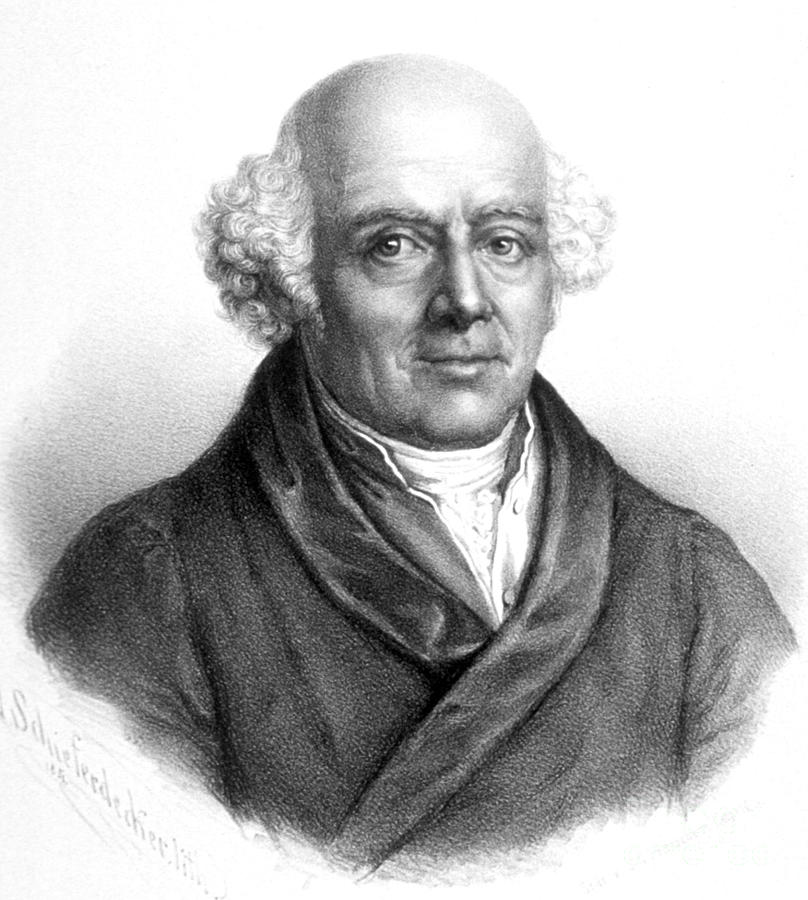
\includegraphics[height=1in]{images/samuel-hahnemann-german-physician-science-source.jpg}
% \end{floatingfigure}

It is not commonly known that Samuel Hahnemann, the originator of
\emph{homeopathy}, did not actually die. In fact, his tomb in P\`ere Lachaise is
empty. After being bitten by a vampire during his return home from dining at \emph{Au
Clairon des Chasseurs}, Hahnemann turned into one as well. From that time on, he
focused on curing the ills of his vampire kin. The fruits of his labors? A
\emph{homeopathic concoction} capable of even raising vampires from the dead.

When a vampire rolls two sixes, a \emph{Midnight}, it is overcome with
compassion for its comrades participating in the Garlic Game. The vampire
administers Hahnemann's homeopathic concoction to the vampires immediately to
the \emph{left} and \emph{right} of the vampire who rolled it. When quaffed, the
concoction \emph{resurrects} vampires who are dead and \emph{sparkles} vampires
who are still alive, strengthening them. The vampires are standing in a
\emph{circle} during the Garlic Game and are numbered from 0 to $n-1$. Vampire 4
has vampire 3 on its left and vampire 5 on its right. What about vampire $n-1$?
It has vampire $n-2$ on its left and vampire $0=n$ on its right. Here is some
code to help calculate the indices of the vampires to the left and right:

\begin{codelisting}{}
//
// Returns the position of the player to the left.
//
// pos: The position of the current player.
// players: The number of players in the game.
//
uint32_t left(uint32_t pos, uint32_t players) {
  return (pos + players - 1) % players;
}

//
// Returns the position of the player to the right.
//
// pos: The position of the current player.
// players: The number of players in the game.
//
uint32_t right(uint32_t pos, uint32_t players) {
  return (pos + 1) % players;
}
\end{codelisting}

Be careful when writing your code to check if a vampire rolled a Midnight. If
rolling a die returns the values 0--5 inclusive, then the maximal sum when
rolling two dice (a Midnight) would be 10. Why not 12? Vampires, like computer
scientists, like to count from \emph{zero}.
\vspace{20pt} % Not sure why the space is missing.

\section{Deliverables}

\epigraph{\emph{Thinking doesn't guarantee that we won't make mistakes. But
not thinking guarantees that we will.}}{---Leslie Lamport}

\noindent You will need to turn in:
\begin{enumerate}
  \item \texttt{vampire.c}: This file will contain your implementation of the
    Garlic Game. The output of your program must match that of the reference
    program's in order to receive full credit.

  \item \texttt{names.h}: This file will be supplied for you and contains the
    naming of the vampires and dice rolls. \textcolor{red}{{Do not change
    this file.}}

  \item \texttt{Makefile}: This is a file that will allow the grader to type
    \texttt{make} to compile your program. Running \texttt{make} or \texttt{make
    all} must build your program. Running \texttt{make clean} must remove any
    compiler-generated files. As this is your first assignment, a working
    \texttt{Makefile} will be supplied for you.

  \item \texttt{README.md}: This must be in \emph{Markdown}. This must describe
    how to build and run your program.

  \item \texttt{DESIGN.pdf}: This \emph{must} be a PDF\@. The design document
    should describe the purpose of your program and communicate its overall
    design with enough detail such that a sufficiently knowledgeable programmer
    would be able to replicate your implementation.  \textcolor{red}{This does
    not mean copying your entire program in verbatim.} You should instead
    describe how your program works with supporting pseudocode.
    \textcolor{red}{\textbf{C} code is \textbf{not} considered pseudocode. You
    \emph{must} push \texttt{DESIGN.pdf} before you push \emph{any} code.}
\end{enumerate}


\section{Submission}

\epigraph{\emph{Calvin: Hocus-pocus abracadabra! I command my homework to do
itself! Homework, be done! Rats.}}{Bill Watterson, \emph{Calvin and Hobbes}}

To submit your assignment through \texttt{git}, refer to the steps shown in
\texttt{asgn0} Remember: \emph{add, commit,} and \emph{push}!
\textcolor{red}{Your assignment is turned in \emph{only} after you have pushed.
If you forget to push, you have not turned in your assignment and you will get a
\emph{zero}. ``I forgot to push'' is not a valid excuse. It is \emph{highly}
recommended to commit and push your changes \emph{often}.}

We will provide you with an \emph{Ubuntu 20.04} binary of our implementation.
Your code should produce \emph{exactly} the same output for \emph{all} inputs in
order to receive full credit.


\section{Supplemental Readings}

\epigraph{\emph{The more that you read, the more things you will know. The
more that you learn, the more places you'll go.}}{---Dr.\ Seuss}

\begin{itemize}
  \item \textit{The C Programming Language} by Kernighan \& Ritchie
  \begin{itemize}
    \item Chapter 3 \S 3.4-3.7
    \item Chapter 4 \S 4.1 \& 4.2
    \item Chapter 7 \S 7.2
    \item Appendix B \S B4
  \end{itemize}
\item \textit{The Kollected Kode Vicious} by George Neville-Neil
\begin{itemize}
\item \S 1.16
\item \S 2.6
\end{itemize}
\end{itemize}

\end{document}
